\documentclass[man,floatsintext]{apa6}
\usepackage{lmodern}
\usepackage{amssymb,amsmath}
\usepackage{ifxetex,ifluatex}
\usepackage{fixltx2e} % provides \textsubscript
\ifnum 0\ifxetex 1\fi\ifluatex 1\fi=0 % if pdftex
  \usepackage[T1]{fontenc}
  \usepackage[utf8]{inputenc}
\else % if luatex or xelatex
  \ifxetex
    \usepackage{mathspec}
  \else
    \usepackage{fontspec}
  \fi
  \defaultfontfeatures{Ligatures=TeX,Scale=MatchLowercase}
\fi
% use upquote if available, for straight quotes in verbatim environments
\IfFileExists{upquote.sty}{\usepackage{upquote}}{}
% use microtype if available
\IfFileExists{microtype.sty}{%
\usepackage{microtype}
\UseMicrotypeSet[protrusion]{basicmath} % disable protrusion for tt fonts
}{}
\usepackage{hyperref}
\hypersetup{unicode=true,
            pdftitle={Who Needs Privacy?},
            pdfauthor={Tobias Dienlin~\& Miriam Metzger},
            pdfkeywords={Privacy, personality, anonymity, integrity, SEM},
            pdfborder={0 0 0},
            breaklinks=true}
\urlstyle{same}  % don't use monospace font for urls
\usepackage{graphicx,grffile}
\makeatletter
\def\maxwidth{\ifdim\Gin@nat@width>\linewidth\linewidth\else\Gin@nat@width\fi}
\def\maxheight{\ifdim\Gin@nat@height>\textheight\textheight\else\Gin@nat@height\fi}
\makeatother
% Scale images if necessary, so that they will not overflow the page
% margins by default, and it is still possible to overwrite the defaults
% using explicit options in \includegraphics[width, height, ...]{}
\setkeys{Gin}{width=\maxwidth,height=\maxheight,keepaspectratio}
\IfFileExists{parskip.sty}{%
\usepackage{parskip}
}{% else
\setlength{\parindent}{0pt}
\setlength{\parskip}{6pt plus 2pt minus 1pt}
}
\setlength{\emergencystretch}{3em}  % prevent overfull lines
\providecommand{\tightlist}{%
  \setlength{\itemsep}{0pt}\setlength{\parskip}{0pt}}
\setcounter{secnumdepth}{0}
% Redefines (sub)paragraphs to behave more like sections
\ifx\paragraph\undefined\else
\let\oldparagraph\paragraph
\renewcommand{\paragraph}[1]{\oldparagraph{#1}\mbox{}}
\fi
\ifx\subparagraph\undefined\else
\let\oldsubparagraph\subparagraph
\renewcommand{\subparagraph}[1]{\oldsubparagraph{#1}\mbox{}}
\fi

%%% Use protect on footnotes to avoid problems with footnotes in titles
\let\rmarkdownfootnote\footnote%
\def\footnote{\protect\rmarkdownfootnote}


  \title{Who Needs Privacy?}
    \author{Tobias Dienlin\textsuperscript{1}~\& Miriam Metzger\textsuperscript{1,2}}
    \date{}
  
\shorttitle{Who Needs Privacy?}
\affiliation{
\vspace{0.5cm}
\textsuperscript{1} University of Hohenheim\\\textsuperscript{2} University of California, Santa Barbara}
\keywords{Privacy, personality, anonymity, integrity, SEM}
\usepackage{csquotes}
\usepackage{upgreek}
\captionsetup{font=singlespacing,justification=justified}

\usepackage{longtable}
\usepackage{lscape}
\usepackage{multirow}
\usepackage{tabularx}
\usepackage[flushleft]{threeparttable}
\usepackage{threeparttablex}

\newenvironment{lltable}{\begin{landscape}\begin{center}\begin{ThreePartTable}}{\end{ThreePartTable}\end{center}\end{landscape}}

\makeatletter
\newcommand\LastLTentrywidth{1em}
\newlength\longtablewidth
\setlength{\longtablewidth}{1in}
\newcommand{\getlongtablewidth}{\begingroup \ifcsname LT@\roman{LT@tables}\endcsname \global\longtablewidth=0pt \renewcommand{\LT@entry}[2]{\global\advance\longtablewidth by ##2\relax\gdef\LastLTentrywidth{##2}}\@nameuse{LT@\roman{LT@tables}} \fi \endgroup}


\usepackage{lineno}

\linenumbers
\setlength{\parskip}{0em}
\raggedbottom

\authornote{Add complete departmental
affiliations for each author here. Each new line herein must be
indented, like this line.

Enter author note here.

Correspondence concerning this article should be addressed to Tobias
Dienlin, University of Hohenheim, Department of Media Psychology (540F).
E-mail:
\href{mailto:tobias.dienlin@uni-hohenheim.de}{\nolinkurl{tobias.dienlin@uni-hohenheim.de}}}

\abstract{
In this study we analyzes how personality relates to
peoples' need for privacy. For example, we analyze if the so-called
\enquote{nothing-to-hide} argument is correct: Do people who lack
integrity really desire more privacy? Moreover, we also analyze the
relation between need for privacy and sociability, anxiety, risk
aversion, and traditionality. Using an online questionnaire with
\emph{N} = 261 mostly student respondents, we found that it is possible
to predict a considerable part of peoples' need for privacy on the basis
of their personalities. For example, we indeed found that repondents who
reported less integrity than others also desired more anonymity.
Moreover, more traditional and more anxious respondents desired more
privacy from the government, while more risk averse and less sociable
respondents desired more privacy from other people. 
}

\usepackage{amsthm}
\newtheorem{theorem}{Theorem}[section]
\newtheorem{lemma}{Lemma}[section]
\theoremstyle{definition}
\newtheorem{definition}{Definition}[section]
\newtheorem{corollary}{Corollary}[section]
\newtheorem{proposition}{Proposition}[section]
\theoremstyle{definition}
\newtheorem{example}{Example}[section]
\theoremstyle{definition}
\newtheorem{exercise}{Exercise}[section]
\theoremstyle{remark}
\newtheorem*{remark}{Remark}
\newtheorem*{solution}{Solution}
\begin{document}
\maketitle















In his novel \emph{The Circle}, Eggers (2013) describes a dystopian
society in which people are gradually forfeiting their privacy. One
after another becomes \enquote{transparent}: Carrying a small camera
around the neck, people begin to broadcast their daily lives to the
Internet. In the novel, this eventually causes a societal upheaval:
\enquote{The pressure on those who hadn't gone transparent went from
polite to oppressive. The question, from pundits and constituents, was
obvious and loud: If you aren't transparent, what are you hiding?}
(Eggers, 2013, p. 129).

With this study, we want to answer the following question. Why do people
desire privacy? To date there is only little research on why people
desire privacy and how the need for privacy can be predicted by aspects
of personality. Why do some people not care whether government agencies
such as the NSA are collecting their data (Greenwald, n.d.), and why do
others protest vehemently in order to protect their privacy?

We think that finding an answer to this question is important: Given
that government agencies are collecting large amounts of data hoping to
reduce criminality and terrorism, and given that government agencies are
collecting this data preemptively and without concrete suspicions, it
seems relevant to find out whether this practice of mass surveillance
can be justified based on the nothing-to-hide argument. As a result, the
main question of this paper is: Do people who desire more privacy really
have more to hide and, more generally, what are personality facets that
determine peoples' overall need for privacy?

\hypertarget{the-need-for-privacy}{%
\subsection{The Need for Privacy}\label{the-need-for-privacy}}

Privacy captures the extent of voluntary withdrawal from others (Westin,
1967). Several models suggest that privacy is a multi-dimensional
concept: For example, in a theory-driven treatise Burgoon (1982) argued
that privacy has four dimensions: informational, social, psychological,
and physical privacy. Pedersen (1979), by contrast, did an empirical
factor analysis (initially starting with 94 items) and suggested that
privacy exists on six dimensions: reserve, isolation, solitude, intimacy
with friends, intimacy with family, and anonymity. In addition, Schwartz
(1968) differentiated between horizontal and vertical privacy: Whereas
horizontal privacy captures withdrawal from peers, vertical privacy
refers to withdrawal from superiors or institutions (e.g., government
agencies).

Next to being multi-dimensional, privacy is also contingent (Dienlin,
2014): One can, for example, distinguish between the objective privacy
context, the subsequent subjective perception of privacy, the
psychological need for privacy (which is both a situational and
dispositional need), and the resulting privacy behavior (as represented
by self-disclosure). For the purpose of this study, we combine the
aforementioned theories and focus on (a) vertical privacy with regard to
the need for withdrawal from government surveillance, (b) horizontal
privacy in terms of the need for withdrawal from peers, friends, or
acquaintances, and (c) both horizontal and vertical privacy as captured
by the general need for anonymity.

\hypertarget{integrity}{%
\subsubsection{Integrity}\label{integrity}}

Which specific aspects of personality help predict need for privacy? The
so-called nothing-to-hide argument states that \enquote{If you have
nothing to hide, you have nothing to fear.} At its core, the
nothing-to-hide argument implies that an important predictor of why
people desire privacy is their \emph{lack of integrity}. This becomes
especially apparent when we consider the definition of Solove's (2007)
nothing-to-hide argument (notably, Solove is a strong critic of the
nothing-to-hide argument):

\begin{quote}
\enquote{The NSA surveillance, data mining, or other government
information gathering programs will result in the disclosure of
particular pieces of information to a few government officials, or
perhaps only to government computers. This very limited disclosure of
the particular information involved is not likely to be threatening to
the privacy of law-abiding citizens. Only those who are engaged in
illegal activities have a reason to hide this information.} (Solove,
2007, p. 753)
\end{quote}

This definition helps illustrate the link between lack of integrity and
need for privacy: People who have \enquote{engaged in illegal
activities} can be considered, by definition, to lack integrity
(Paunonen, 2002), which is why they have a reason \enquote{to hide this
information} (or, in other words, to desire more privacy). In terms of a
scientific definition of integrity there is no real consensus, however
most scholars agree that integrity \enquote{incorporates a tendency to
comply with social norms, avoid deviant behavior, and embrace a sense of
justice, truthfulness, and fairness} (Connelly, Lilienfeld, \& Schmeelk,
2006, p. 82).

Several theoretical arguments exist why lack of integrity might
correlate with need for privacy. In general, any self-disclosure is a
potential risk because others might disagree, disapprove, or misuse the
information in other contexts (Petronio, 2010). Privacy regulation
theory showed that if self-disclosures are too risky, people raise their
desired level of privacy, intensify their boundary regulation, and
employ more mechanisms to seclude and protect themselves (Altman, 1976).
In traditional contexts, this could range from moderate behaviors like
closing doors, to extreme behaviors such as physically tossing someone
out of the room (Altman, 1976). In modern contexts, protecting one's
privacy can mean to avoid photographs or to deliberately shun public
places that have surveillance cameras. People who have actually
committed something bad, treacherous, or illegal become even more
vulnerable and face a significant risk of self-disclosure, because
others will surely disapprove of these activities (Petronio, 2010).
Hence, the foregoing arguments illuminate an indirect link between
integrity and need for privacy: By definition, people who participate in
negative activities are considered to lack integrity (Paunonen, 2002).
People who have engaged in negative activities have, by definition, more
to hide, and disclosures concerning those activities pose a high risk.
Because of this increased risk, people will arguably desire more
privacy, as a means to mitigate their felt risk (Altman, 1976). In this
way, the current research extends Altman's privacy regulation theory
(1976) by suggesting that lack of integrity is an important yet
unexamined factor that could increase peoples' desired level of privacy.

A few studies can be found that imply a relation between privacy and
integrity. For example, several studies found that surveillance reduces
cheating behaviors (Corcoran \& Rotter, 1987, Covey.1989). Covey,
Saladin, and Killen (1989) asked students to solve an impossible maze.
In the high surveillance condition, the experimenter stood in front of
the students and closely monitored their behavior. In the low
surveillance condition, the experimenter stood behind the students, did
not monitor their behavior, and visual dividers were used to block the
experimenter's view of the students. Results showed that students were
more likely to cheat in the low surveillance condition, suggesting that
in situations of surveillance (i.e., less privacy), people show fewer
cheating behaviors (i.e., more integrity). Similarly, people are more
likely to prevent others from stealing when security cameras are visible
(van Bommel, van Prooijen, Elffers, \& van Lange, 2014), which is also a
sign of higher integrity. Next, in a longitudinal sample with 457
respondents in Germany (Trepte, Dienlin, \& Reinecke, 2013), people who
reported needing more privacy were less satisfied with their lives
(\emph{r} = -.47), had more (\emph{r} = .41) and less positive affect
(\emph{r} = -.39). More importantly however, people who felt they needed
more privacy were also less authentic on their SNSs profiles (\emph{r} =
-.48) and less authentic in their personal relationships (\emph{r} =
-.28; Trepte et al., 2013). For example, people who agreed to items like
\enquote{I do not talk about personal issues unless my conversation
partner brings them up first} were more likely to report that their
online profiles did not truly represent their personality. Given the
argument that authenticity is a subset of integrity (Sheldon, 2004), we
reason that the concept of integrity might relate to the desired level
of privacy. Finally, Pedersen (1982) showed that three dimensions of
need for privacy related to self-esteem: In his study with \emph{N} = 70
undergraduate students, respondents who held a lower self-esteem were
more reserved (\emph{r} = .29), needed more anonymity (\emph{r} = .21)
and preferred solitude (\emph{r} = .24). Granted, self-esteem and
integrity are generally distinct concepts; however, Pedersen's specific
operationalization of self-esteem integrated several aspects of
integrity (e.g., by using items such as \enquote{moral, nice, fair,
unselfish, good, honest, reputable, sane} to measure self-esteem). Thus,
our overarching hypothesis is that people who lack integrity have a
greater need for privacy.

In accordance with the reasoning mentioned above, we suggest that people
with less integrity feel a greater need for privacy. Specifically, we
argue that integrity may relate to the need for privacy from (a)
government surveillance, as governments have the legitimate power to
prosecute illegal activities. Next, we hypothesize that integrity
relates to the desire privacy for (b) anonymity. Anonymity makes it more
difficult for both legal and social agents to identify and address
potential wrongdoers, which is why people with less integrity will
prefer situations in which they are anonymous. Finally, lack of
integrity likely also relates to an increased need for privacy from (c)
other people, as most other people will disapprove of immoral or illegal
activities, and might reveal those activities to authorities.

Hypothesis 1: People who feel lower in self-perceived integrity desire
more privacy from government surveillance (H1a), more anonymity (H1b),
and more privacy from other people (H1c).

\hypertarget{sociability}{%
\subsubsection{Sociability}\label{sociability}}

Critics of the nothing-to-hide argument hold that people who desire
privacy should not automatically be confronted with suspicion, and that
privacy has several purposes that are not related to criminal behavior
(Marlinspike, n.d.). Westin (1967), for example, defined four primary
purposes of privacy: (1) self-development (i.e., the integration of
experiences into meaningful patterns), (2) autonomy (i.e., the desire to
avoid being manipulated and dominated), (3) emotional release (i.e., the
release of tension from social role demands), and (4) protected
communication (i.e., the ability to foster intimate relationships).
These are all important social factors for which people desire privacy.
Hence, the argument is that people who desire privacy can have several
legitimate reasons for doing so; reasons which are essential for
psychosocial wellbeing and which relate to different factors of
personality. Below, we thus explore other (neutral) aspects of
personality that potentially predict need for privacy. In order to be
more precise, we follow the advice by Paunonen and Ashton (2001) and,
instead of using generic personality factors as predictors, refer to
specific personality facets.

First, we argue that people who are more reserved, who feel less
comfortable in social situations, generally desire more anonymity and
more interpersonal privacy. Given that privacy is, by definition, a
voluntary withdrawal from society (Westin, 1967), we expect that people
who are more reserved or more shy desire more privacy from others.
Several empirical studies support this hypothesis: Extroverted people
desire less privacy (Morton, 2013), people who describe themselves as
introverted thinkers are more likely to prefer social isolation
(Pedersen, 1982), and introverted people are more likely to report
invasions of privacy (Stone, 1986). Finally, we did not find convincing
theoretical and empirical arguments for why sociability should relate to
an increased need for privacy from government surveillance, which is why
we did not include a hypothesis on this relation.

Hypothesis 2: People who are more sociable desire less anonymity (H2a)
and less privacy from other people (H2b).

\hypertarget{anxiety}{%
\subsubsection{Anxiety}\label{anxiety}}

Of course, there are also reasons why people might desire less privacy.
Government agencies often curtail privacy with the aim to prevent crime:
For example, the NSA's surveillance programs are often considered a
direct response to the 9 / 11 terrorists attacks (Greenwald, n.d.). It
seems plausible that people who are more afraid of terrorist attacks are
also more likely to consent to these surveillance programs, given that
these programs promise to reduce the likelihood of future attacks. One
can then argue that people who are afraid of terrorist attacks are also
more afraid of threats overall, which is why we suggest that people who
are, in general, more anxious desire less privacy from government
surveillance and less anonymity. We did not include a hypothesis on the
potential relation between anxiety and need for interpersonal privacy.
On the one hand, one could argue that people who are more anxious are
more reserved, given that social interactions can pose significant risks
(especially with strangers or weak ties; Granovetter, 1973). At the same
time, one could suggest that especially those people who are more
anxious desire less privacy from others (and especially their strong
ties), in order to cope better with their daily challenges. At the end,
given that we measure interpersonal privacy on a general level (and do
not distinguish between need for privacy from (a) weak ties and (b)
strong ties), it seems plausible that both effects could cancel each
other out.

Hypothesis 3: People who are more anxious desire less privacy from
government surveillance (H3a) and more anonymity (H3b).

\hypertarget{risk-aversion}{%
\subsubsection{Risk aversion}\label{risk-aversion}}

Disclosing personal information always poses a certain risk, given that
others can misuse self-disclosed personal information in different
contexts, which can lead to severe consequences (Altman, 1976). Not
everyone will feel intimidated by this hypothetical threat---except
those who have a general tendency to avoid taking unnecessary risks. The
most cautious strategy to minimize risks of personal self-disclosures
would be, arguably, to keep as much information as possible private.
Hence, we suggest that people who are, in general, more risk averse have
a good reason to desire more privacy in all three aforementioned
contexts.

Hypothesis 4: People who are more risk averse desire more privacy from
government surveillance (H4a), more anonymity (H4b), and more privacy
from other people (H4c).

\hypertarget{traditionality}{%
\subsubsection{Traditionality}\label{traditionality}}

The personal computer and the Internet have rendered the world
increasingly digitized: Social interactions, purchases, and medical
treatments nowadays all produce digital traces, which can be combined
into accurate latent user profiles. Given the features of digital
information (i.e., information is persistent, searchable, reproducible,
and scalable; boyd, 2008), this allows for unprecedented ways and
degrees of surveillance. Mark Zuckerberg famously observed that privacy
is no longer a \enquote{social norm,} rather that people share personal
information (Johnson, n.d.). Hence, in order to be part of contemporary
life (e.g., by using SNSs), it seems necessary to give up some privacy.
However, arguably not everyone is willing to pay that price, and
especially people who are more conservative might prefer to stick to
their usual routines and decide against giving up their privacy. This is
supported by empirical research: Older people, who are generally less
open and more traditional (Donnellan \& Lucas, 2008), are more concerned
about their privacy than younger people (Fife \& Orjuel, 2012). Taken
together, we suggest that people who are more traditional also desire
more privacy in all three aforementioned contexts.

Hypothesis 5: People who are more traditional desire more privacy from
government surveillance (H5a), more anonymity (H5b), and more privacy
from other people (H5c).

\hypertarget{sociodemographic-variables}{%
\subsubsection{Sociodemographic
variables}\label{sociodemographic-variables}}

(Dear Miriam, I would like to add a short paragraph on how
sociodemographics relate to privacy. Relevant studies I can think of are
Park (2015), Tifferet (2019), Weinberger, Zhitomirsky-Geffet, and
Bouhnik (2017), Trepte et al. (2013). I haven't yet managed to write it,
maybe you have time?)

\hypertarget{methods}{%
\section{Methods}\label{methods}}

We report how we determined our sample size, all data exclusions (if
any), all manipulations, and all measures in the study.

\hypertarget{open-science}{%
\subsection{Open science}\label{open-science}}

The following information can be found in the online supplementary
material (OSM): the data, the study material, the syntax, unabridged
results, additional analyses, and a reproducible version of the
manuscript. Next to the variables reported here, we also collected
additional ones, which can be found in the OSM. We invite everyone to
for example rerun our analyses or to investigate novel research
questions. It is also possible to suggest changes and/or corrections to
the manuscript. The OSM can be found here:
\url{https://github.com/tdienlin/need_for_privacy/}.

\hypertarget{data-analyses}{%
\subsection{Data analyses}\label{data-analyses}}

All hypotheses were tested with a two-tailed significance level of 5\%.
Regarding effect sizes, we classified regression coefficients with
values exceeding \(\upbeta\) = .10 as small effects, \(\upbeta\) = .30
as medium effects, and \(\upbeta\) = .50 as large effects. In that vein,
our smallest effect size of interest (SESOI; Lakens, Scheel, \& Isager,
2018) was \(\upbeta\) = .10. Effects below the SESOI are considered too
small to be theoretically relevant.

We removed participants with peculiar response patterns (e.g.,
straight-linining, missing of inverted items). As criterion, we used the
Guttman value, which allows to identify respondents with peculiar
response patterns (Meijer, Niessen, \& Tendeiro, 2016). We individually
inspected respondents whose reponses were most extreme (5\% quantile).
Indeed, these reponses showed either obvious response patterns, which is
why these 5\% were excluded from the analyses. Next, we excluded one
participant who provided an illogical age (i.e., 9 years). We also
excluded all respondents who anwered less than 50\% of all questions.
The remaining missing responses were imputed using predictive mean
matching. No respondents needed to be exluded due to \enquote{speeding}
(i.e., \textless{} 5 minutes answer time).

The factorial validity of the measures and the hypotheses were tested
with structural equation modeling (SEM). Mardia's test showed that the
assumption of multivariate normality was violated, \emph{p}(skewness)
\textless{} .001, \emph{p}(kurtosis) \textless{} .001. As a result, we
used the more robust Satorra-Bentler scaled and mean-adjusted test
statistic (MLM) as estimator. Fit was assessed using the conventional
measures and criteria as proposed by Kline (2016).

First, by running confirmatory factor analyses we tested the factorial
validity of the variables we collected. In a first step, we ran
exploratory factor analyses to assess the underlying factor structure.
If more than one factor was found, we ran exploratory factor analyses
looking for a bifactor model solution. Bifactor models implement one
factor that explains the variance in all items (the so-called general
factor or g-factor). Next, at least two more additional factors are
implemented that explain the variance in a subset of the items. The
general factor and the specific factors are orthogonal. Bifactor models
are nested within hierachical models and are in general more liberal
than hierachical models. For more information on bifactor models, see
Kline (2016). If the bifactor model did not show sufficient factorial
validity, we proceeded by deleting items with low loadings on the
general factor and/or the specific factors. If no bifactor solution
could be found, using a subset of the items we then aimed to extract a
single factor with sufficient factorial validity.

To test our hypotheses, we regressed the dependent variable need for
privacy unto the predictor variables. To increase parsimonity, the
predictor variables were not modelled as latent factors. Instead, using
the model predicted values of the CFAs we computed factor score for each
respondent. If the CFAs showed a single-factor solution, we used the
model predicted values for this latent factor; if the CFAs produced a
bifactor solution, we used the model predicted values for the general
latent factor.

The criterion, need for privacy, was measured as latent construct. In
general, combining the information of several items into a general
latent construct helps reduce and combine information, which allows for
more robust and precise inferences. At the same time, there are several
degrees of freedom regarding how to exactly specify general latent
constructs. In light of our not having preregistered the analyses, in
order to provide the complete picture we hence also report how the
independent variables predicted each item measuring need for privacy
individually (see Figure \ref{fig:results-items}).

We used R (Version 3.5.1; R Core Team, 2018) and the R-packages
\emph{ggplot2} (Version 3.1.0; Wickham, 2016), \emph{lavaan} (Version
0.6.3; Rosseel, 2012), \emph{papaja} (Version 0.1.0.9842; Aust \& Barth,
2018), \emph{semPlot} (Version 1.1; Epskamp \& Simon Stuber, 2017), and
\emph{tidyverse} (Version 1.2.1; Wickham, 2017) for all our analyses.

\hypertarget{procedure-and-participants}{%
\subsection{Procedure and
participants}\label{procedure-and-participants}}

Participants were students from a university in the western U.S. who
received course credit for taking part in the study. The initial sample
consisted of \emph{N} = 296 respondents. After the removing of the
defective data, the final sample consisted of \emph{N} = 261
respondents. The age ranged from 18 to 56 years (\emph{M} = 20 years),
with 27\% of the respondents being male. The median participation time
was 5.22min.

The study was run in 2015. At the time we were not yet aware of the
importance to run a-priori power analyses to determine sample size. It
was our aim to collect a large number of participants (i.e., \emph{N} =
300). The final sample size allowed to find effects with a size of
\(\upbeta\) = 0.22 in 95\% of all cases. We had a power to detect small
effects (i.e., \(\upbeta\) = .10) in 36\% of all cases.

\hypertarget{measures}{%
\subsection{Measures}\label{measures}}

In what follows we present how we operationalized our constructs. First,
it was possible to model all variables with at least acceptable fit.
Note that all items were answered on a 7-point Likert scale ranging from
1 (\emph{strongly disagree}) to 7 (\emph{strongly agree}). For an
overview of the items' psychometrics, factorial validity, and
reliability, see Table \ref{tab:psychometrics}. The data, all items
(including deleted ones), results of CFAs, item statistics, and
distribution plots can be found in the OSM.

\begin{table}[tbp]
\begin{center}
\begin{threeparttable}
\caption{\label{tab:psychometrics}Psychometrics of Variables Used.}
\footnotesize{
\begin{tabular}{lllllllllllll}
\toprule
 & \multicolumn{1}{c}{m} & \multicolumn{1}{c}{sd} & \multicolumn{1}{c}{chisq} & \multicolumn{1}{c}{df} & \multicolumn{1}{c}{pvalue} & \multicolumn{1}{c}{cfi} & \multicolumn{1}{c}{tli} & \multicolumn{1}{c}{rmsea} & \multicolumn{1}{c}{srmr} & \multicolumn{1}{c}{omega} & \multicolumn{1}{c}{alpha} & \multicolumn{1}{c}{ave}\\
\midrule
Privacy need & 4.17 & 1.61 & 107.36 & 62.00 & < .001 & .95 & .93 & .05 & .05 & .84 & .89 & .47\\
Integrity & 4.56 & 1.81 & 50.81 & 23.00 & < .001 & .95 & .92 & .07 & .05 & .79 & .82 & .40\\
Sociability & 4.67 & 1.48 & 12.77 & 3.00 & .005 & .97 & .85 & .11 & .04 & .78 & .83 & .51\\
Anxiety & 4.40 & 1.50 & 29.60 & 16.00 & .020 & .97 & .94 & .06 & .04 & .80 & .83 & .44\\
Risk aversion & 4.34 & 1.51 & 33.13 & 16.00 & .007 & .95 & .91 & .06 & .05 & .74 & .80 & .42\\
Traditionality & 3.89 & 1.57 & 13.73 & 5.00 & .017 & .95 & .91 & .08 & .04 & .73 & .73 & .35\\
\bottomrule
\addlinespace
\end{tabular}
}
\begin{tablenotes}[para]
\normalsize{\textit{Note.} All items were measured on 7-point scales with Likert response options. Alpha = Cronbach's alpha (internal consistency); omega = Raykov's omega (composite reliability); ave = average variance extracted.}
\end{tablenotes}
\end{threeparttable}
\end{center}
\end{table}

\hypertarget{need-for-privacy}{%
\subsubsection{Need for privacy}\label{need-for-privacy}}

As main variable of interest, we collected several items to measure the
need for privacy. First, we collected 4 items capturing the need for
\emph{informational privacy} using the scale by Trepte and Masur (2017).
One example items was \enquote{I prefer it when other people do not know
much about me.}

Second, we measured the need for privacy on a \emph{societal} level
using 9 self-designed items. The first subdimension was \emph{government
surveillance}, which represents the extent to which people want the
government to abstain from collecting information about their personal
life. One example item is \enquote{I feel the need to protect my privacy
from government agencies.} The second dimension was \emph{anonymity},
which measures the extent to which people feel the need to avoid
identification (\enquote{I prefer not to carry my ID with me all the
time to preserve my privacy}).

Third, we measured the need for privacy on a \emph{interpersonal} level
using 9 self-designed items. The first subdimension measured the need
for privacy from other people in \emph{online contexts}. One example
items was \enquote{I don't feel the need to be able to communicate about
very personal things with others online}. The second subdimension
measured the need for privacy from other people in \emph{offline
contexts}. One example item was \enquote{I don't feel the need to tell
my friends all my secrets}.

Exploratory and confirmatory factor analyses finally revealed a
well-fitting bifactor model, which consisted of one general factor
measuring a general need for privacy and three specific ones measuring
the need for privacy from the government, the need for privacy from
other people, and the need for anonymity. For a list of all items, see
Table \ref{tab:need-for-privacy-items}. For an overview of the items'
loadings in the final bifactor model, see Figure
\ref{fig:need-for-privacy-loadings}.

\begin{figure}
\centering
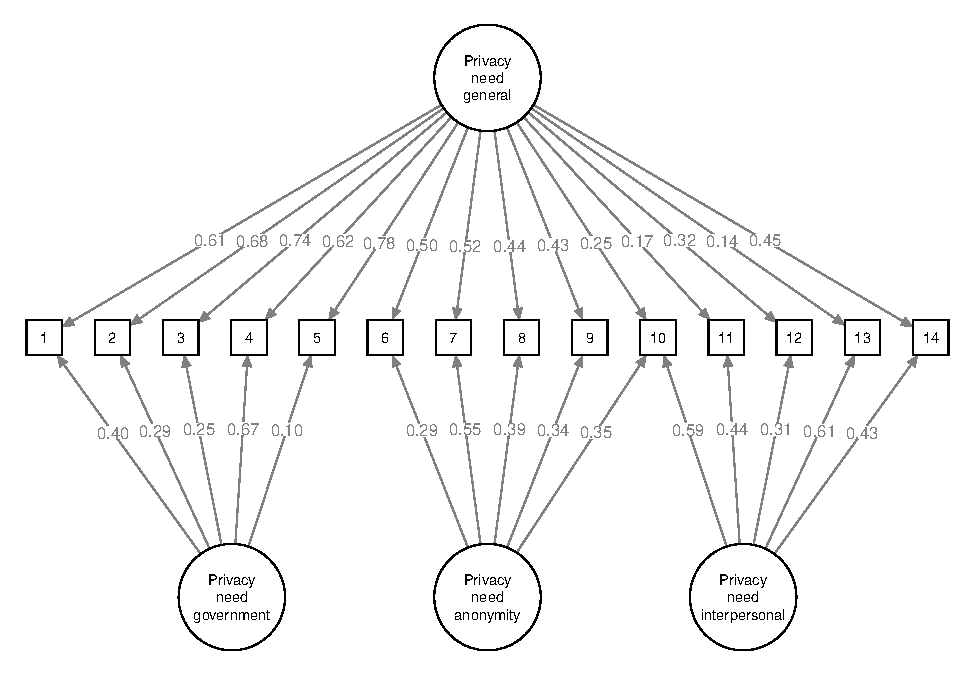
\includegraphics{manuscript_files/figure-latex/need-for-privacy-loadings-1.pdf}
\caption{\label{fig:need-for-privacy-loadings}Overview of the bifactor model
for the need for privacy}
\end{figure}

\newpage

\begin{table}

\caption{\label{tab:need-for-privacy-items}Overview of the Items Measuring the Need for Privacy}
\centering
\resizebox{\linewidth}{!}{
\fontsize{7}{9}\selectfont
\begin{tabular}[t]{ll>{\raggedright\arraybackslash}p{10cm}}
\toprule
Name & No. & Content\\
\midrule
N4P.SOC\_1 & 1 & I need government agencies to respect my privacy, even if that hinders a greater societal cause.\\
N4P.SOC\_2 & 2 & I need the information that companies (e.g., Amazon, Facebook, or Google) have about me to stay private so that the government can never access it.\\
N4P.SOC\_3 & 3 & I don’t want the government to gather information about me, even if that makes it more difficult for them to spend tax income efficiently.\\
N4P.SOC\_4 & 4 & I don’t want government agencies to monitor my personal communication, even if doing so prevents future terrorist attacks.\\
N4P.SOC\_5 & -- & I need to be able to surf online anonymously.\\
N4P.SOC\_6 & 6 & I need to be able to use a fake name on social network sites to preserve my privacy.\\
N4P.SOC\_7 & 7 & I feel the need to avoid places with video surveillance.\\
N4P.SOC\_8 & 8 & I prefer not to carry my ID with me all the time to preserve my privacy.\\
N4P.SOC\_9 & 5 & I feel the need to protect my privacy from government agencies.\\
N4P.INT\_1 & -- & I feel the need to disclose personal information about me on social network sites.\\
N4P.INT\_2 & 9 & My need for privacy is so strong that it prevents me from using Facebook actively.\\
N4P.INT\_3 & -- & I don’t feel the need to be able to communicate about very personal things with others online.\\
N4P.INT\_4 & 12 & I need to know that my boss or future employers cannot find information about me online that they might disapprove of.\\
N4P.INT\_5 & -- & I always need a person to talk about personal things.\\
N4P.INT\_6 & -- & I don’t need to know a lot of things about people I interact with, as that might cause problems.\\
N4P.INT\_7 & 13 & I don’t feel the need to tell my friends all my secrets.\\
N4P.INT\_8 & -- & I sometimes feel the need to share my personal point of view with someone I don’t know that well.\\
N4P.INT\_9 & 14 & I feel the need to protect my privacy from other people.\\
N4P.BOT\_1 & 10 & I prefer it when other people do not know much about me.\\
N4P.BOT\_2 & -- & When given the chance, I prefer being incognito.\\
N4P.BOT\_3 & 11 & I don’t want personal information about me being publicly available.\\
N4P.BOT\_4 & -- & Not everybody needs to know everything about me.\\
\bottomrule
\end{tabular}}
\end{table}

\hypertarget{integrity-1}{%
\subsubsection{Integrity}\label{integrity-1}}

Integrity measures the extent to which people comply with culturally
established norms and values. In order to measure lack of integrity, we
used the subscale \emph{integrity} of the Supernumerary Personality
Inventory (Paunonen, 2002), which consists of 8 items. In addition, we
self-designed another three items. An example item is \enquote{I don't
think there's anything wrong with cheating a little on one's income tax
forms.} Analyses revealed that a bifactor model based on a subset of 9
items showed good fit to the data.

\hypertarget{sociability-1}{%
\subsubsection{Sociability}\label{sociability-1}}

Sociability captures whether people prefer to spend their time alone or
in company. We measured sociability with the extraversion subscale
\emph{gregariousness} (John \& Srivastava, 1999), which consists of 8
items. An example item is \enquote{I shy away from crowds of people.}
Analyses revealed that a bifactor model based on a subset of 6 items
showed good fit to the data.

\hypertarget{anxiety-1}{%
\subsubsection{Anxiety}\label{anxiety-1}}

Anxiety measures whether people are afraid of negative external
influences. We measured anxiety with the neuroticism subscale
\emph{anxiety} (John \& Srivastava, 1999), which consists of 8 items. An
example item is \enquote{I am easily frightened.} Analyses revealed that
a bifactor model using all 8 items showed good fit to the data.

\hypertarget{risk-avoidance}{%
\subsubsection{Risk avoidance}\label{risk-avoidance}}

Risk avoidance captures whether people abstain from taking risks. We
measured risk avoidance with the conscientiousness subscale
\emph{deliberation} (John \& Srivastava, 1999), which consists of 8
items. An example item is \enquote{I think twice before I answer a
question.} Analyses revealed that a bifactor model using all 8 items
showed good fit to the data.

\hypertarget{traditionalism}{%
\subsubsection{Traditionalism}\label{traditionalism}}

Traditionalism measures whether people prefer to stick with their usual
routines. We measured traditionalism with the (inverted) openness to
experiences subscale \emph{actions} (John \& Srivastava, 1999), which
consists of 8 items. An example item is \enquote{I'm pretty set in my
ways.} Analyses revealed that a model with a single factor based on a
subset of 5 items showed good fit to the data.

\hypertarget{results}{%
\section{Results}\label{results}}

In what follows, we present the verbatim result. For the exact
statistical results, see Table \ref{tab:results}. For visualization of
the results by means of confidence intervals, see Figure
\ref{fig:results-factor}.

\begin{table}[tbp]
\begin{center}
\begin{threeparttable}
\caption{\label{tab:results}Results of the main factorial model.}
\scriptsize{
\begin{tabular}{lrrrrr}
\toprule
Predictor & \multicolumn{1}{c}{b} & \multicolumn{1}{c}{ll} & \multicolumn{1}{c}{ul} & \multicolumn{1}{c}{beta} & \multicolumn{1}{c}{p}\\
\midrule
Privacy need general &  &  &  &  & \\
\ \ \ Integrity & -0.24 & -0.48 & 0.01 & -.15 & .062\\
\ \ \ Sociability & -0.16 & -0.44 & 0.13 & -.09 & .289\\
\ \ \ Anxiety & -0.01 & -0.20 & 0.18 & -.01 & .897\\
\ \ \ Traditionalism & -0.12 & -0.30 & 0.06 & -.12 & .190\\
\ \ \ Risk avoidance & 0.77 & -0.19 & 1.73 & .14 & .117\\
\ \ \ Male & 0.18 & -0.12 & 0.48 & .10 & .233\\
\ \ \ Age & 0.04 & 0.01 & 0.07 & .14 & .006\\
\ \ \ Income & 0.04 & -0.08 & 0.17 & .05 & .495\\
Privcacy need government &  &  &  &  & \\
\ \ \ Integrity & 0.16 & -0.15 & 0.47 & .10 & .316\\
\ \ \ Sociability & -0.15 & -0.55 & 0.24 & -.09 & .440\\
\ \ \ Anxiety & -0.27 & -0.49 & -0.04 & -.26 & .019\\
\ \ \ Traditionalism & 0.42 & 0.14 & 0.69 & .43 & .003\\
\ \ \ Risk avoidance & -0.06 & -1.16 & 1.04 & -.01 & .920\\
\ \ \ Male & 0.03 & -0.34 & 0.40 & .02 & .881\\
\ \ \ Age & -0.02 & -0.06 & 0.01 & -.08 & .174\\
\ \ \ Income & -0.01 & -0.16 & 0.14 & -.01 & .891\\
Privacy need interpersonal &  &  &  &  & \\
\ \ \ Integrity & 0.24 & 0.01 & 0.48 & .15 & .039\\
\ \ \ Sociability & -0.62 & -0.90 & -0.34 & -.34 & < .001\\
\ \ \ Anxiety & 0.01 & -0.16 & 0.17 & .01 & .938\\
\ \ \ Traditionalism & 0.25 & 0.05 & 0.44 & .23 & .012\\
\ \ \ Risk avoidance & 1.01 & 0.06 & 1.96 & .17 & .038\\
\ \ \ Male & -0.02 & -0.30 & 0.26 & -.01 & .899\\
\ \ \ Age & < 0.01 & -0.03 & 0.04 & .02 & .764\\
\ \ \ Income & -0.03 & -0.16 & 0.10 & -.04 & .621\\
Privacy need anonymity &  &  &  &  & \\
\ \ \ Integrity & -0.19 & -0.38 & 0.01 & -.23 & .061\\
\ \ \ Sociability & -0.08 & -0.28 & 0.12 & -.10 & .423\\
\ \ \ Anxiety & -0.04 & -0.14 & 0.06 & -.08 & .448\\
\ \ \ Traditionalism & 0.03 & -0.09 & 0.15 & .05 & .654\\
\ \ \ Risk avoidance & -0.29 & -0.89 & 0.31 & -.10 & .351\\
\ \ \ Male & 0.13 & -0.07 & 0.33 & .15 & .193\\
\ \ \ Age & -0.01 & -0.04 & 0.02 & -.04 & .673\\
\ \ \ Income & 0.07 & -0.03 & 0.18 & .18 & .149\\
\bottomrule
\end{tabular}
}
\end{threeparttable}
\end{center}
\end{table}

\begin{figure}
\centering
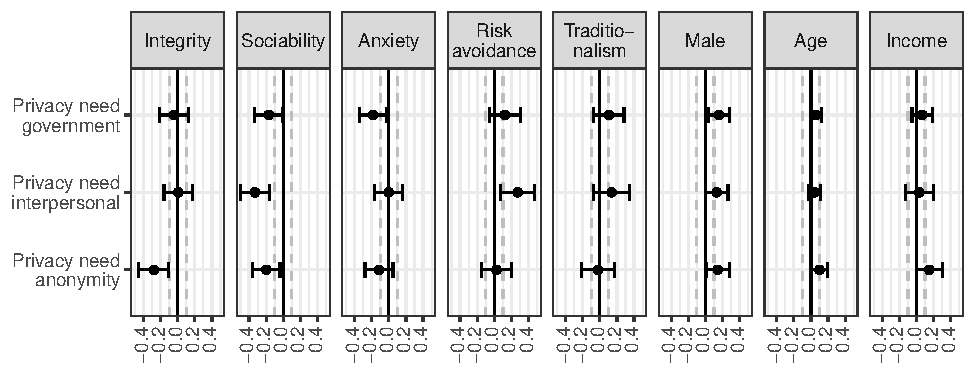
\includegraphics{manuscript_files/figure-latex/results-factor-1.pdf}
\caption{\label{fig:results-factor}Overview of results. Shows the 95\%
confidence intervals of standardized coefficients.}
\end{figure}

To begin with, we found that the final model we estimated to test our
hypotheses fit the data moderately well, \(\chi^2\)(142) = 233.64,
\textit{p} \textless{} .001, cfi = .92, rmsea = .05, 90\% CI {[}.04,
.06{]}, srmr = .05. Our first hypothesis stated that people reporting
more integrity than others would need less privacy. Indeed, the results
showed that respondents who reported more integrity than others desired
moderately less anonymity. The relation with general privacy showed the
same relation; however, it was marginally not significant.
Interestingly, respondents who reported more integrity desired
\emph{more} privacy from other people. No significant relation with the
need for privacy from the government was found.

Respondents who reported being more sociable than other desired less
privacy from other people. The effect was of a considerable size. No
other significant relations were found.

Next, we found that respondents who indicated being more anxious than
others also desired less privacy from the government. The effect size
was moderate to considerable. No other significnat relations were found.

Respondents who reported being more risk avoidant than others desired
moderately more privacy from other people. No further significant
effects were found.

Next, respondents who indicated being more traditional than others also
desired more privacy from the government. The effect was substantial.
More traditional respondents also desired moderately more privacy from
other people. No significant relations with the overall level of privacy
and the need for anonymity were found.

Finally, regarding sociodemographic variables, we found that respondents
who were older also desired more privacy. The effect was small.

In sum, the predictors could explained 8.82\% of the variance in the
general need for privacy, 23.06\% of the variance in the need for
privacy from the government, 29.71\% of the variance in the need for
privacy from other people, and 15.52\% of the variance in the need for
anonymity.

As stated above, we also calculated the relation between the predictor
variables and the individual privacy need items. Several significant
relations were found. For a visualization, see Figure
\ref{fig:results-items}.

\begin{figure}
\centering
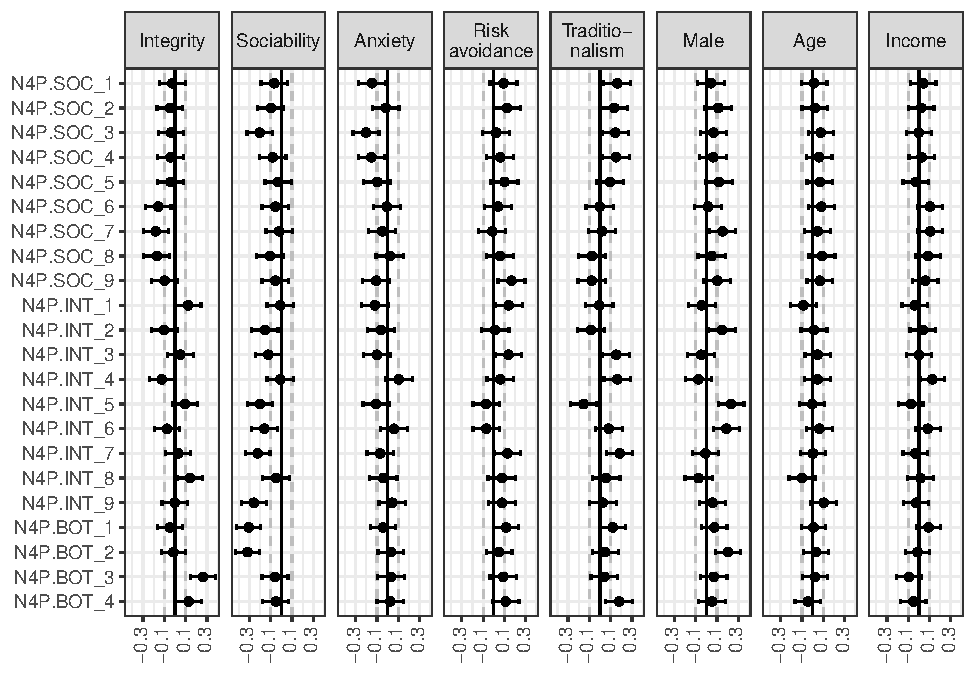
\includegraphics{manuscript_files/figure-latex/results-items-1.pdf}
\caption{\label{fig:results-items}Overview of results. Shows the 95\%
confidence intervals of standardized coefficients.}
\end{figure}

\hypertarget{discussion}{%
\section{Discussion}\label{discussion}}

This study analyzed how the need for privacy can be predicted by means
of personality. In a study with 261 students from a large US university,
we measured the need for privacy with 22 items. Fifteen items formed a
well-fitting bifactor model, with one factor measuring the general
desire for privacy, and three specific factors measuring the need for
privacy from the government, the need for privacy from other people, and
the need for anonymity. The factor solution we found is in line with
privacy theory, which subsumes a vertical level (here, privacy from the
government) and a horizontal level (here, privacy from other people).
The third dimension, need for anonymity, can be argued to exist on the
diagonal, as one can be anonymous both from the government and from
other people.

The results showed that the need for privacy can be predicted
considerably well by means of personality. Specifically, integrity
relates to several dimensions of need for privacy: People who reported
being of lower integrity desired more anonymity and slightly less
privacy from other people. Respondents who said, for example, that they
would feel tempted to take things that do not belong to them were also
more likely to avoid situations in which they were identifiable.

In conclusion, our results follow Altman (1976), who reasoned that if
exposure of information is risky it is likely that people will use more
mechanisms to strengthen their social boundaries and increase their
desired level of privacy. This study thus aligns with Altman's privacy
regulation theory by showing that, in several contexts, people with
lower integrity had a higher level of desired privacy.

In addition, need for privacy was predicted also by other (neutral)
personality facets: People who were less sociable, more risk averse, and
less anxious also desired more privacy. This implies that various
personality-related aspects can predict need for privacy.

People who are more shy, more risk averse, or less anxious also desire
more privacy. For example, people who are more anxious are more likely
to accept government surveillance (arguably because they are less afraid
of terrorist attacks). When looking at the bigger implications of the
results, this shows the importance to make differentiated claims on why
people desire privacy: Indeed, the results suggest that some people
desire privacy because they might have something to hide. However,
putting everyone who desires privacy under a general suspicion is wrong
given that less sociable, risk averse, and less anxious people are also
more likely to desire privacy.

As a side note, despite the fact that we mostly used well-established
scales, confirmatory factor analyses (CFAs) showed that some of the
original items had to be deleted in order to achieve adequate factorial
validity. This resembles the finding by Hussey and Hughes (2018), who
reported that several widely used scales in psychological research
actually do not show high factorial validity. We would like to point out
that by using bifactor models it is possible to at least partially
alleviate the problem, as the bifactor models are less strict than the
routinely used unidimensional or hierarchical models, which are more
conservative.

\hypertarget{limitations-and-future-perspective}{%
\subsection{Limitations and future
perspective}\label{limitations-and-future-perspective}}

Power analyses showed that future research should use samples above
\emph{N} \(\approx\) 260 in order to test hypotheses with the
recommended power of at least .80 (Cohen (1992)).

In general, the question arises whether it is possible, or even socially
desirable, to measure a person's integrity. On the one hand, integrity
implies absolute criteria: Stealing is bad and forbidden, whereas
helping is good and encouraged. On the other hand, integrity implies
relative criteria: Whereas some cultures disapprove of lying whatever
the context, others consider lying okay---for example \enquote{white
lies} in order to save face or to avoid hurting someone's feelings
(Altman, 1977). Thus, ranking behaviors, opinions, and character traits
with regard to integrity is a moral dilemma. As a result, throughout the
entire study we have understood integrity as a transgression of social
norms that is strong and that most societies would agree upon (for
example, most societies would consider stealing as a sign of low
integrity).

Next, the question arises whether it is possible to measure integrity
based on self-reports. Interestingly, integrity tests using self-reports
have been shown to work successfully, given that they can predict
unwanted professional workplace behavior sufficiently (e.g., theft, drug
and alcohol problems, or absenteeism; Ones, Viswesvaran, \& Schmidt,
1993). In a meta-analysis with 665 correlation coefficients, integrity
tests related to counterproductive behaviors with a coefficient of
\emph{r} = .47 (Ones et al., 1993). Nonetheless, future research would
benefit from including behavioral manifestations of integrity, such as
concrete cheating behaviors. If concrete cheating behaviors also
increase desires for privacy, this would strengthen the underlying
premise of the nothing-to-hide argument.

In that vein, we decided against including social desirability as a
control variable, because even though social desirability can affect
answers to sensitive questions (de Jong, Pieters, \& Stremersch, 2012),
it is arguably more likely to reflect a true personality trait than
false answering behavior (de Vries, Zettler, \& Hilbig, 2014).

By focusing on \emph{specific facets} of personality (e.g.,
fearfulness), we followed the recommendation by Paunonen and Ashton
(2001) to not analyze \emph{general factors} of personality (e.g.,
neuroticism). For future research, we suggest going one step further by
analyzing predictors that are even more specified. For example, it seems
possible that people who hold dissenting political beliefs could also
have a higher need for privacy from the government. Similarly, it would
be interesting to focus on different minority groups. For example, it
seems plausible that people from a LGBT background might desire more
privacy from government (because it is potentially repressive or
unfriendly toward LGBTs). Finally, in this study we focused mostly on
escapist motives for why people desire privacy (e.g., sociability, risk
aversion). Interestingly, Leary, Herbst, and McCrary (2003) were able to
show that when predicting engagement in solitary activities, it is less
preferable to measure how strongly people want to escape society
(avoidance oriented), but rather how much they seek solitude (approach
oriented). Hence, future studies might want to include predictors that
are more approach oriented (e.g., peoples' need for contemplation).

From a methodological perspective, future research should continue to
improve the instruments we used, given that factorial validity of some
scales was only moderate. Similarly, we recommend elaborating on the
general understanding of integrity as a theoretical concept. To date,
there is not one overarching concept of integrity that incorporates all
the different aspects of integrity, yet it would be valuable to examine
how other aspects of integrity (e.g., authenticity, trustworthiness, or
consistency) relate to privacy desires.

Optimizing the variables' factorial validity might introduce problems of
overfitting. In other words, although we might now have a sharper knife,
we also use it less situations. First, we think that by using bifactor
models we were able to retain a large number of items, rendering our
results more robust. In addition, also when looking at the items
individually one can see that the results are not dependent on inclusion
of specific items.

\hypertarget{conclusion}{%
\subsection{Conclusion}\label{conclusion}}

\newpage

\hypertarget{references}{%
\section{References}\label{references}}

\begingroup
\setlength{\parindent}{-0.5in}
\setlength{\leftskip}{0.5in}

\hypertarget{refs}{}
\leavevmode\hypertarget{ref-Altman.1976}{}%
Altman, I. (1976). Privacy: A conceptual analysis. \emph{Environment and
Behavior}, \emph{8}(1), 7--29.
doi:\href{https://doi.org/10.1177/001391657600800102}{10.1177/001391657600800102}

\leavevmode\hypertarget{ref-Altman.1977}{}%
Altman, I. (1977). Privacy regulation: Culturally universal or
culturally specific? \emph{Journal of Social Issues}, \emph{33}(3),
66--84.
doi:\href{https://doi.org/10.1111/j.1540-4560.1977.tb01883.x}{10.1111/j.1540-4560.1977.tb01883.x}

\leavevmode\hypertarget{ref-R-papaja}{}%
Aust, F., \& Barth, M. (2018). \emph{papaja: Create APA manuscripts with
R Markdown}. Retrieved from \url{https://github.com/crsh/papaja}

\leavevmode\hypertarget{ref-boyd.2008c}{}%
boyd, danah m. (2008). \emph{Taken out of context. American teen
sociality in networked publics: Doctoral dissertation}. Berkeley, CA:
University of California.

\leavevmode\hypertarget{ref-Burgoon.1982}{}%
Burgoon, J. K. (1982). Privacy and communication. \emph{Annals of the
International Communication Association}, \emph{1}, 206--249.

\leavevmode\hypertarget{ref-Cohen.1992}{}%
Cohen, J. (1992). A power primer. \emph{Psychological Bulletin},
\emph{112}(1), 155--159.
doi:\href{https://doi.org/10.1037/0033-2909.112.1.155}{10.1037/0033-2909.112.1.155}

\leavevmode\hypertarget{ref-Connelly.2006}{}%
Connelly, S., Lilienfeld, S. O., \& Schmeelk, K. M. (2006). Integrity
tests and morality: Associations with ego development, moral reasoning,
and psychopathic personality. \emph{International Journal of Selection
and Assessment}, \emph{14}(1), 82--86.
doi:\href{https://doi.org/10.1111/j.1468-2389.2006.00335.x}{10.1111/j.1468-2389.2006.00335.x}

\leavevmode\hypertarget{ref-Corcoran.1987}{}%
Corcoran, K. J., \& Rotter, J. B. (1987). Morality-conscience guilt
scale as a predictor of ethical behavior in a cheating situation among
college females. \emph{The Journal of General Psychology},
\emph{114}(2), 117--123.
doi:\href{https://doi.org/10.1080/00221309.1987.9711061}{10.1080/00221309.1987.9711061}

\leavevmode\hypertarget{ref-Covey.1989}{}%
Covey, M. K., Saladin, S., \& Killen, P. J. (1989). Self-monitoring,
surveillance, and incentive effects on cheating. \emph{The Journal of
Social Psychology}, \emph{129}(5), 673--679.
doi:\href{https://doi.org/10.1080/00224545.1989.9713784}{10.1080/00224545.1989.9713784}

\leavevmode\hypertarget{ref-deJong.2012}{}%
de Jong, M. G., Pieters, R., \& Stremersch, S. (2012). Analysis of
sensitive questions across cultures: An application of multigroup item
randomized response theory to sexual attitudes and behavior.
\emph{Journal of Personality and Social Psychology}, \emph{103}(3),
543--564. doi:\href{https://doi.org/10.1037/a0029394}{10.1037/a0029394}

\leavevmode\hypertarget{ref-deVries.2014}{}%
de Vries, R. E., Zettler, I., \& Hilbig, B. E. (2014). Rethinking trait
conceptions of social desirability scales: Impression management as an
expression of honesty-humility. \emph{Assessment}, \emph{21}(3),
286--299.
doi:\href{https://doi.org/10.1177/1073191113504619}{10.1177/1073191113504619}

\leavevmode\hypertarget{ref-Dienlin.2014}{}%
Dienlin, T. (2014). The privacy process model. In S. Garnett, S. Halft,
M. Herz, \& J. M. Mönig (Eds.), \emph{Medien und Privatheit} (pp.
105--122). Passau, Germany: Karl Stutz.

\leavevmode\hypertarget{ref-Donnellan.2008}{}%
Donnellan, M. B., \& Lucas, R. E. (2008). Age differences in the Big
Five across the life span: Evidence from two national samples.
\emph{Psychology and Aging}, \emph{23}(3), 558--566.
doi:\href{https://doi.org/10.1037/a0012897}{10.1037/a0012897}

\leavevmode\hypertarget{ref-Eggers.2013}{}%
Eggers, D. (2013). \emph{The circle}. New York, NY: Knopf Publishing
Group.

\leavevmode\hypertarget{ref-R-semPlot}{}%
Epskamp, S., \& Simon Stuber. (2017). \emph{SemPlot: Path diagrams and
visual analysis of various sem packages' output}. Retrieved from
\url{https://CRAN.R-project.org/package=semPlot}

\leavevmode\hypertarget{ref-Fife.2012}{}%
Fife, E., \& Orjuel, J. (2012). The privacy calculus: Mobile apps and
user perceptions of privacy and security. \emph{International Journal of
Engineering Business Management}, \emph{4}, 1--10.
doi:\href{https://doi.org/10.5772/51645}{10.5772/51645}

\leavevmode\hypertarget{ref-Granovetter.1973}{}%
Granovetter, M. S. (1973). The strength of weak ties. \emph{American
Journal of Sociology}, \emph{78}(6), 1360--1380.

\leavevmode\hypertarget{ref-Greenwald.2013}{}%
Greenwald, G. (n.d.). NSA collecting phone records of millions of
Verizon customers daily. \emph{The Guardian}. Retrieved from
\url{www.theguardian.com}

\leavevmode\hypertarget{ref-Hussey.2018}{}%
Hussey, I., \& Hughes, S. (2018). Hidden invalidity among fifteen
commonly used measures in social and personality psychology.
doi:\href{https://doi.org/10.31234/osf.io/7rbfp}{10.31234/osf.io/7rbfp}

\leavevmode\hypertarget{ref-John.1999}{}%
John, O. P., \& Srivastava, S. (1999). The big five trait taxonomy:
History, measurement, and theoretical perspectives. In L. A. Pervin \&
O. P. John (Eds.), \emph{Handbook of personality} (pp. 102--138). New
York, NY: Guilford Press.

\leavevmode\hypertarget{ref-Johnson.2010}{}%
Johnson, B. (n.d.). Privacy no longer a social norm, says Facebook
founder. \emph{The Guardian}. Retrieved from \url{www.theguardian.com}

\leavevmode\hypertarget{ref-Kline.2016}{}%
Kline, R. B. (2016). \emph{Principles and practice of structural
equation modeling} (4th ed.). New York, NY: The Guilford Press.

\leavevmode\hypertarget{ref-Lakens.2018}{}%
Lakens, D., Scheel, A. M., \& Isager, P. M. (2018). Equivalence testing
for psychological research: A tutorial. \emph{Advances in Methods and
Practices in Psychological Science}, \emph{1}(2), 259--269.
doi:\href{https://doi.org/10.1177/2515245918770963}{10.1177/2515245918770963}

\leavevmode\hypertarget{ref-Leary.2003}{}%
Leary, M. R., Herbst, K. C., \& McCrary, F. (2003). Finding pleasure in
solitary activities: Desire for aloneness or disinterest in social
contact? \emph{Personality and Individual Differences}, \emph{35}(1),
59--68.
doi:\href{https://doi.org/10.1016/S0191-8869(02)00141-1}{10.1016/S0191-8869(02)00141-1}

\leavevmode\hypertarget{ref-Marlinspike.2013}{}%
Marlinspike, M. (n.d.). Why 'I have nothing to hide' is the wrong way to
think about surveillance. Retrieved from \url{www.wired.com}

\leavevmode\hypertarget{ref-Meijer.2016}{}%
Meijer, R. R., Niessen, A. S. M., \& Tendeiro, J. N. (2016). A practical
guide to check the consistency of item response patterns in clinical
research through person-fit statistics: Examples and a computer Program.
\emph{Assessment}, \emph{23}(1), 52--62.
doi:\href{https://doi.org/10.1177/1073191115577800}{10.1177/1073191115577800}

\leavevmode\hypertarget{ref-Morton.2013}{}%
Morton, A. (2013). Measuring inherent privacy concern and desire for
privacy - A pilot survey study of an instrument to measure dispositional
privacy concern. In \emph{International Conference on Social Computing
(SocialCom)} (pp. 468--477).
doi:\href{https://doi.org/10.1109/SocialCom.2013.73}{10.1109/SocialCom.2013.73}

\leavevmode\hypertarget{ref-Ones.1993}{}%
Ones, D. S., Viswesvaran, C., \& Schmidt, F. L. (1993). Comprehensive
meta-analysis of integrity test validities: Findings and implications
for personnel selection and theories of job performance. \emph{Journal
of Applied Psychology}, \emph{78}(4), 679--703.
doi:\href{https://doi.org/10.1037/0021-9010.78.4.679}{10.1037/0021-9010.78.4.679}

\leavevmode\hypertarget{ref-Park.2015}{}%
Park, Y. J. (2015). Do men and women differ in privacy? Gendered privacy
and (in)equality in the Internet. \emph{Computers in Human Behavior},
\emph{50}, 252--258.
doi:\href{https://doi.org/10.1016/j.chb.2015.04.011}{10.1016/j.chb.2015.04.011}

\leavevmode\hypertarget{ref-Paunonen.2002}{}%
Paunonen, S. V. (2002). Design and construction of the Supernumerary
Personality Inventory. London, Canada: University of Western Ontario.

\leavevmode\hypertarget{ref-Paunonen.2001}{}%
Paunonen, S. V., \& Ashton, M. C. (2001). Big Five factors and facets
and the prediction of behavior. \emph{Journal of Personality and Social
Psychology}, \emph{81}(3), 524--539.
doi:\href{https://doi.org/10.1037/0022-3514.81.3.524}{10.1037/0022-3514.81.3.524}

\leavevmode\hypertarget{ref-Pedersen.1979}{}%
Pedersen, D. M. (1979). Dimensions of privacy. \emph{Perceptual and
Motor Skills}, \emph{48}(3), 1291--1297.
doi:\href{https://doi.org/10.2466/pms.1979.48.3c.1291}{10.2466/pms.1979.48.3c.1291}

\leavevmode\hypertarget{ref-Pedersen.1982}{}%
Pedersen, D. M. (1982). Personality correlates of privacy. \emph{The
Journal of Psychology}, \emph{112}(1), 11--14.
doi:\href{https://doi.org/10.1080/00223980.1982.9923528}{10.1080/00223980.1982.9923528}

\leavevmode\hypertarget{ref-Petronio.2010}{}%
Petronio, S. (2010). Communication privacy management theory: What do we
know about family privacy regulation? \emph{Journal of Family Theory \&
Review}, \emph{2}(3), 175--196.
doi:\href{https://doi.org/10.1111/j.1756-2589.2010.00052.x}{10.1111/j.1756-2589.2010.00052.x}

\leavevmode\hypertarget{ref-R-base}{}%
R Core Team. (2018). \emph{R: A language and environment for statistical
computing}. Vienna, Austria: R Foundation for Statistical Computing.
Retrieved from \url{https://www.R-project.org/}

\leavevmode\hypertarget{ref-R-lavaan}{}%
Rosseel, Y. (2012). lavaan: An R package for structural equation
modeling. \emph{Journal of Statistical Software}, \emph{48}(2), 1--36.
Retrieved from \url{http://www.jstatsoft.org/v48/i02/}

\leavevmode\hypertarget{ref-Schwartz.1968}{}%
Schwartz, B. (1968). The social psychology of privacy. \emph{American
Journal of Sociology}, \emph{73}(6), 741--752.

\leavevmode\hypertarget{ref-Sheldon.2004}{}%
Sheldon, K. M. (2004). Integrity {[}authenticity, honesty{]}. In C.
Peterson \& Seligman, M. E. P. (Eds.), \emph{Character strengths and
virtues: A handbook and classification} (pp. 249--271). Oxford, UK:
Oxford University Press.

\leavevmode\hypertarget{ref-Solove.2007}{}%
Solove, D. J. (2007). 'I've got nothing to hide' and other
misunderstandings of privacy. \emph{San Diego Law Review}, \emph{44},
745--772.

\leavevmode\hypertarget{ref-Stone.1986}{}%
Stone, D. L. (1986). Relationship between introversion/extraversion,
values regarding control over information, and perceptions of invasion
of privacy. \emph{Perceptual and Motor Skills}, \emph{62}(2), 371--376.
doi:\href{https://doi.org/10.2466/pms.1986.62.2.371}{10.2466/pms.1986.62.2.371}

\leavevmode\hypertarget{ref-Tifferet.2019}{}%
Tifferet, S. (2019). Gender differences in privacy tendencies on social
network sites: A meta-analysis. \emph{Computers in Human Behavior},
\emph{93}, 1--12.
doi:\href{https://doi.org/10.1016/j.chb.2018.11.046}{10.1016/j.chb.2018.11.046}

\leavevmode\hypertarget{ref-Trepte.2013a}{}%
Trepte, S., Dienlin, T., \& Reinecke, L. (2013). Privacy,
self-disclosure, social support, and social network site use. Research
report of a three-year panel study. Retrieved from
\url{http://opus.uni-hohenheim.de/volltexte/2013/889/}

\leavevmode\hypertarget{ref-Trepte.2017d}{}%
Trepte, S., \& Masur, P. K. (2017). Need for privacy. In V. Zeigler-Hill
\& T. K. Shackelford (Eds.), \emph{Encyclopedia of Personality and
Individual Differences} (Vol. 94, pp. 1--4). Cham: Springer
International Publishing.
doi:\href{https://doi.org/10.1007/978-3-319-28099-8_540-1}{10.1007/978-3-319-28099-8\_540-1}

\leavevmode\hypertarget{ref-vanBommel.2014}{}%
van Bommel, M., van Prooijen, J.-W., Elffers, H., \& van Lange, P. A. M.
(2014). Intervene to be seen: The power of a camera in attenuating the
bystander effect. \emph{Social Psychological and Personality Science},
\emph{5}(4), 459--466.
doi:\href{https://doi.org/10.1177/1948550613507958}{10.1177/1948550613507958}

\leavevmode\hypertarget{ref-Weinberger.2017b}{}%
Weinberger, M., Zhitomirsky-Geffet, M., \& Bouhnik, D. (2017). Sex
differences in attitudes towards online privacy and anonymity among
Israeli students with different technical backgrounds, \emph{22}(4).
Retrieved from \url{http://InformationR.net/ir/22-4/paper777.html}

\leavevmode\hypertarget{ref-Westin.1967}{}%
Westin, A. F. (1967). \emph{Privacy and freedom}. New York, NY:
Atheneum.

\leavevmode\hypertarget{ref-R-ggplot2}{}%
Wickham, H. (2016). \emph{Ggplot2: Elegant graphics for data analysis}.
Springer-Verlag New York. Retrieved from \url{http://ggplot2.org}

\leavevmode\hypertarget{ref-R-tidyverse}{}%
Wickham, H. (2017). \emph{Tidyverse: Easily install and load the
'tidyverse'}. Retrieved from
\url{https://CRAN.R-project.org/package=tidyverse}

\endgroup


\end{document}
